\documentclass[12pt,a4paper,titlepage]{article}
\usepackage[utf8]{inputenc}
\usepackage[T1]{fontenc}
\usepackage[french]{babel}
\usepackage{graphicx}
\usepackage{amsthm}
\usepackage{amsmath, amsfonts}
\usepackage{amssymb}
\usepackage{mathrsfs}
\usepackage{color}
\usepackage{colortbl}
\usepackage{url}
\usepackage{color}
\usepackage{listings}

\title{OS13 : Tests d'estimation et lois extrêmes des lois de Cauchy et géométrique}
\author{\textsc{Adrien WARTELLE} \\ \textsc{TRAN Quoc Nhat Han}}
\date{\today}
\lstset{
language=R,
basicstyle=\scriptsize\ttfamily,
commentstyle=\ttfamily\color{green},
numbers=left,
numberstyle=\ttfamily\color{black}\footnotesize,
stepnumber=1,
numbersep=5pt,
backgroundcolor=\color{white},
showspaces=false,
showstringspaces=false,
showtabs=false,
frame=single,
tabsize=2,
captionpos=b,
breaklines=true,
breakatwhitespace=false,
keywordstyle=\color{blue},
stringstyle=\color{magenta},
literate=
  {á}{{\'a}}1 {é}{{\'e}}1 {í}{{\'i}}1 {ó}{{\'o}}1 {ú}{{\'u}}1
  {Á}{{\'A}}1 {É}{{\'E}}1 {Í}{{\'I}}1 {Ó}{{\'O}}1 {Ú}{{\'U}}1
  {à}{{\`a}}1 {è}{{\`e}}1 {ì}{{\`i}}1 {ò}{{\`o}}1 {ù}{{\`u}}1
  {À}{{\`A}}1 {È}{{\'E}}1 {Ì}{{\`I}}1 {Ò}{{\`O}}1 {Ù}{{\`U}}1
  {ä}{{\"a}}1 {ë}{{\"e}}1 {ï}{{\"i}}1 {ö}{{\"o}}1 {ü}{{\"u}}1
  {Ä}{{\"A}}1 {Ë}{{\"E}}1 {Ï}{{\"I}}1 {Ö}{{\"O}}1 {Ü}{{\"U}}1
  {â}{{\^a}}1 {ê}{{\^e}}1 {î}{{\^i}}1 {ô}{{\^o}}1 {û}{{\^u}}1
  {Â}{{\^A}}1 {Ê}{{\^E}}1 {Î}{{\^I}}1 {Ô}{{\^O}}1 {Û}{{\^U}}1
  {œ}{{\oe}}1 {Œ}{{\OE}}1 {æ}{{\ae}}1 {Æ}{{\AE}}1 {ß}{{\ss}}1
  {ű}{{\H{u}}}1 {Ű}{{\H{U}}}1 {ő}{{\H{o}}}1 {Ő}{{\H{O}}}1
  {ç}{{\c c}}1 {Ç}{{\c C}}1 {ø}{{\o}}1 {å}{{\r a}}1 {Å}{{\r A}}1
  {€}{{\EUR}}1 {£}{{\pounds}}1
}
\numberwithin{equation}{section}

\definecolor{mygreen}{RGB}{28,172,0} % color values Red, Green, Blue
\definecolor{mylilas}{RGB}{170,55,241}
\lstset{language=Matlab,%
    %basicstyle=\color{red},
    breaklines=true,%
    morekeywords={matlab2tikz},
    keywordstyle=\color{blue},%
    morekeywords=[2]{1}, keywordstyle=[2]{\color{black}},
    identifierstyle=\color{black},%
    stringstyle=\color{mylilas},
    commentstyle=\color{mygreen},%
    showstringspaces=false,%without this there will be a symbol in the places where there is a space
    numbers=left,%
    numberstyle={\tiny \color{black}},% size of the numbers
    numbersep=9pt, % this defines how far the numbers are from the text
    emph=[1]{for,end,break},emphstyle=[1]\color{red}, %some words to emphasise
    %emph=[2]{word1,word2}, emphstyle=[2]{style},    
}

\begin{document}
\maketitle 
\renewcommand{\contentsname}{Sommaire}
\tableofcontents

\clearpage

\begin{abstract}
Ce rapport montre comment estimer des paramètres pour la loi géométrique et la loi de Cauchy.
On y étudie aussi les lois extrêmes correspondantes.
\end{abstract}

\section{Loi géométrique}

\subsection{Rappel}

La loi géomètrique est une loi discrète utilisée
dans le cadre d'un enchainement (non fini) d'épreuves de Bernouilli. Soit
$X$ une variable aléatoire suivant cette loi $G(p)$, on a:
\[P(X=k) = (1-p)^{k-1}p\ \ ,k\in\mathbb{N}_{+}\]
La variable X correspond au numéro de la première épreuve où l'on obtient un succès, celle-ci ayant une probabilité p. Ainsi, p est le seul paramètre de la loi.
La fonction de répartition $F(k) = P(X\leq{}k)\ (k\in\mathbb{N}_{+})$ est:
\[F(k)=1-(1-p)^{k}\]
\begin{proof}
On peut remarquer que:
\[P(X=k)=(1-p)^{k-1}(1-(1-p))=(1-p)^{k-1}-(1-p)^{k}\]
Donc :
\[F(k)=\sum\limits_{l=1}^{k}P(X=l)=\sum\limits_{l=1}^{k}((1-p)^{l-1}-(1-p)^{l})\]
\[F(k)=\sum\limits_{l=0}^{k-1}(1-p)^{l}-\sum\limits_{l=1}^{k}(1-p)^{l}\]
Soit $q=1-p$, on a :
\[F(k)=\sum\limits_{l=0}^{k-1}q^{l}-\sum\limits_{l=1}^{k}q^{l}\]
\[F(k)=\frac{1-q^k}{1-q}-(\frac{1-q^{k+1}}{1-q}-1)\]
\[F(k)=\frac{1-q^k-1+q^{k+1}+1-q}{1-q}\]
\[F(k)=\frac{1-q+q^{k+1}-q^k}{1-q}\]
\[F(k)=\frac{1-q-q^k(1-q)}{1-q}\]
\[F(k)=1-q^k\]
On retrouve bien :
\[F(k)=1-(1-p)^k\]
\end{proof}

\subsection{Génération de n variables aléatoires}

Afin de voir à quoi ressemble la distribution et de pouvoir tester l'estimateur que
nous allons calculer par la suite, on génère des échantillons de 50, 500 et 5000 variables.
On utilise ainsi le code Matlab (Octave) ci-dessous :

\lstinputlisting[language=Matlab, firstline=3, lastline=28]{src/geom.m}

On obtient ainsi la figure \ref{Histogrammes et distribution de loi géométrique}.

\begin{figure}[!h]
\begin{center}
 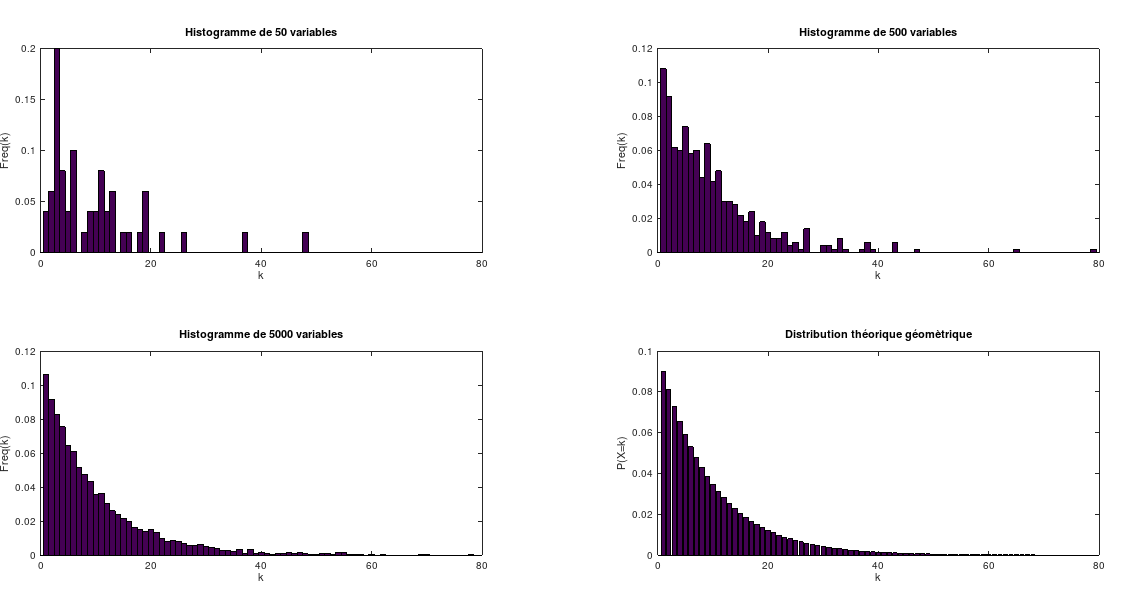
\includegraphics[scale=0.4]{images/histGeom.png} 
\end{center}
 \caption{Histogrammes et distribution de loi géométrique}
 \label{Histogrammes et distribution de loi géométrique}
\end{figure}

On observe bien que les histogrammes se rapprochent de la distribution théorique quand
la taille de l'échantillon est grande (plusieurs milliers). On peut aussi noter que la distribution
se rapproche d'une loi exponentielle (qui a pour distribution $f(t)=\lambda e^{-\lambda t}, \forall x \in \mathbb{R}_{+}$). En effet la loi géométrique est aussi une loi sans mémoire, c'est-à-dire que :
\[\forall k,l \in \mathbb{N}_{+}, P(X=k+l|X>k) = P(X=l) = (1-p)^{l-1}p \]
Cette propriété caractérise la loi exponentielle dans le cas continue, on voit alors que la loi exponentielle correspond à la limite continue de la loi géométrique si l'on fait correspondre les valeurs k obtenues par $X\sim G(p)$ avec des intervalles de  $\mathbb{R}_{+}$ et si l'on fait correspondre $p$ avec la probabilité $P(t_{k}<T<t_{k}+h|t_{k})=e^{-\lambda h}$, T suivant une loi exponentielle $\epsilon(\lambda)$ et $[t_{k},t_{k}+h]$ l'intervalle correspondant à la valeur k. Pour améliorer cette "similarité", on prendra $h$ et (donc $p$) le plus petit possible.

Pour générer les populations , on utilise la fonction "geomGen" qui simule
n expériences où, pour chacune d'entre elle, on effectue un enchainement
d'épreuves de Bernouilli en générant une variable de loi uniforme sur
$[0;1]$ . Si la valeur obtenu est supérieure à p, ce qui a une probabilité p d'arriver, on arrête la boucle
et la valeur générée est égale au nombre d'épreuves, sinon on continue 
jusqu'à obtenir cette condition. Le code Matlab (Octave) utilisé est :

\lstinputlisting[language=Matlab]{src/geomGen.m}

Cette méthode revient à générer de manière répéter
une variable de Bernouilli.


\subsection{Estimateurs du maximum de vraisemblance}

L'estimateur $\hat{p}$ du maximum de vraisemblance est la valeur qui
maximise la loi de vraisemblance L(p) : $\hat{p}=arg\ \underset{p}{max}(L(p))$.
On calcule L(p) dans un premier temps en assumant que les variables sont indépendantes \footnote{on le supposera par la suite pour les échantillons générés} :
\[L(p)=L(X_1(p),X_2(p),...,X_n(p))=\prod\limits_{i=1}^{n}(1-p)^{X_i-1}p 
\]
avec $X_i,\ i\in\{1,..,n\}$ les variables d'échantillon.
\[L(p)=p^n(1-p)^{(\sum\limits_{i=1}^{n}X_i)-n}\]
On peut effectuer un passage au logarithme pour trouver un maximum car il s'agit
d'une fonction strictement croissante (et défini sur $]0;1]$). L'argument du maximum du logarithme
de $L(p)$ et du maximum de $L(p)$ sont les mêmes.
\[\log{L(p)}=n\log{p}+((\sum\limits_{i=1}^{n}X_i)-n)\log{(1-p)}\]
\[\frac{d\log{L(p)}}{dp}=\frac{n}{p}-\frac{(\sum\limits_{i=1}^{n}X_i)-n}{1-p}\]
\[\text{On a }\frac{d\log{L(\hat{p})}}{dp}=0\]
\[\text{Donc }\frac{n-n\hat{p}-((\sum\limits_{i=1}^{n}X_i)-n)\hat{p}}{\hat{p}(1-\hat{p})}=0\]
\[\text{Ce qui implique (dans le cas différent de 0 et 1) }n-(\sum\limits_{i=1}^{n}X_i)\hat{p}=0\]
Finalement :
\[\hat{p} = \frac{n}{\sum\limits_{i=1}^{n}X_i}\]
De plus on peut vérifier qu'il s'agit bien d'un maximum (unique et donc global) en regardant si la fonction $L(p)$ est concave :
\[\frac{d^2\log{L(p)}}{dp^2} = -\frac{n}{p^2}-\frac{\sum\limits_{i=1}^{n}X_i-n}{(1-p)^2}\]
Sachant que $\sum\limits_{i=1}^{n}X_i > n $
et que $p\in[0;1]$, on a:
\[\frac{d^2 \log{L(p)}}{dp^2}<0 \ \forall p\in[0;1]\]
La fonction $L(p)$ est donc concave et l'estimateur trouvé $\hat{p} = \frac{n}{\sum\limits_{i=1}^{n}X_i}$ maximise bien la loi de vraisemblance.

Si la résolution analytique pour trouver l'estimateur avait été impossible,
l'utilisation d'un algorithme d'optimisation de vraisemblance (comme une descente de gradient par exemple) ou encore
l'utilisation d'une fonction intégrée à R ou Matlab aurait été possible.

\subsection{Test de l'estimateur}

Afin de tester l'estimateur du maximum de vraisemblance pour différent taille
d'échantillon, on utilise le code suivant :

\lstinputlisting[language=Matlab]{src/deltaEstGeom.m}

On estime la valeur théorique $p=0.1$ en utilisant
estimateur de vraisemblance $\hat{p} = \frac{n}{\sum\limits_{i=1}^{n}X_i}$ pour des tailles d'échantillons $n$ allant de 10 à 10000.
On mesure pour chaque $n$ l'écart relatif $\frac{\hat{p}-p}{p}$ et on obtient la figure \ref{Evolution du biais de l'estimateur geom}.

\begin{figure}[!h]
\begin{center}
 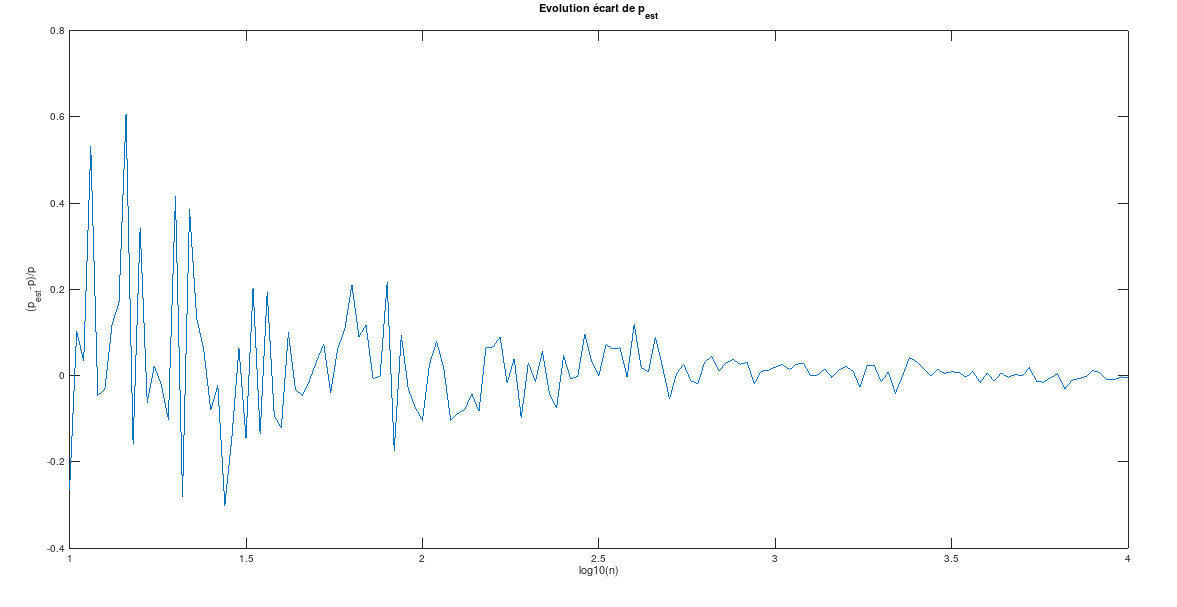
\includegraphics[scale=0.3]{images/biaisGeom.png} 
\end{center}
 \caption{Evolution du biais de l'estimateur}
 \label{Evolution du biais de l'estimateur geom}
\end{figure}

On voit que que l'estimateur commence à être relativement précis, c'est à dire avec un biais relatif en dessous de 10\%, autour de 1000 ($10^3$ valeurs) variables générées. On peut noter aussi que, pour des valeurs petites de n, les écarts sont beaucoup plus souvent positifs ($\hat{p}>p$) que négatifs ($\hat{p}<p$) et que ces écarts positifs vont jusqu'à plus de 60\% alors que les négatifs sont en dessous de 35\%. On peut alors émettre l'hypothèse que notre estimateur est biaisé (plutôt positivement) pour des valeurs de n inférieures à 1000. 

Pour confirmer cette hypothèse, il faudrait calculer le biais de l'estimateur qui correspond à l'écart moyen (d'espérance) entre l'estimateur et le paramètre réel. En effet l'écart entre $p$ et $\hat{p}$ est une variable aléatoire qui va dépendre de l'échantillon généré\footnote{Il faut donc plusieurs échantillons pour le tester (pour un n donné)}. Si on essaye d'obtenir une valeur théorique :
\[B=\mathbb{E}(\hat{p} - p)\]
\[B=\mathbb{E}(\hat{p}) - p\]
\[B=n\mathbb{E}\left(\frac{i=1}{\sum\limits_{1}^{n}X_{i}}\right) - p\]

On voit que ce calcul n'est pas simple puisqu'il
faudrait connaître la loi de l'inverse de la somme de variables géométriques (ou tout du moins son espérance). 

Nous allons donc estimer l'espérance du biais, pour différentes valeurs de n, en utilisant la moyenne des biais obtenus sur plusieurs échantillons (pour une même taille n) :

\lstinputlisting[language=Matlab]{src/deltaEspEstGeom.m}

Pour des valeurs de n allant de 10 à 1000, on calcule l'écart moyen de 500 estimations provenant de 500 échantillons différents et obtient la figure\ref{Evolution de l'écart moyen de de l'estimateur geom}.

\begin{figure}[!h]
\begin{center}
 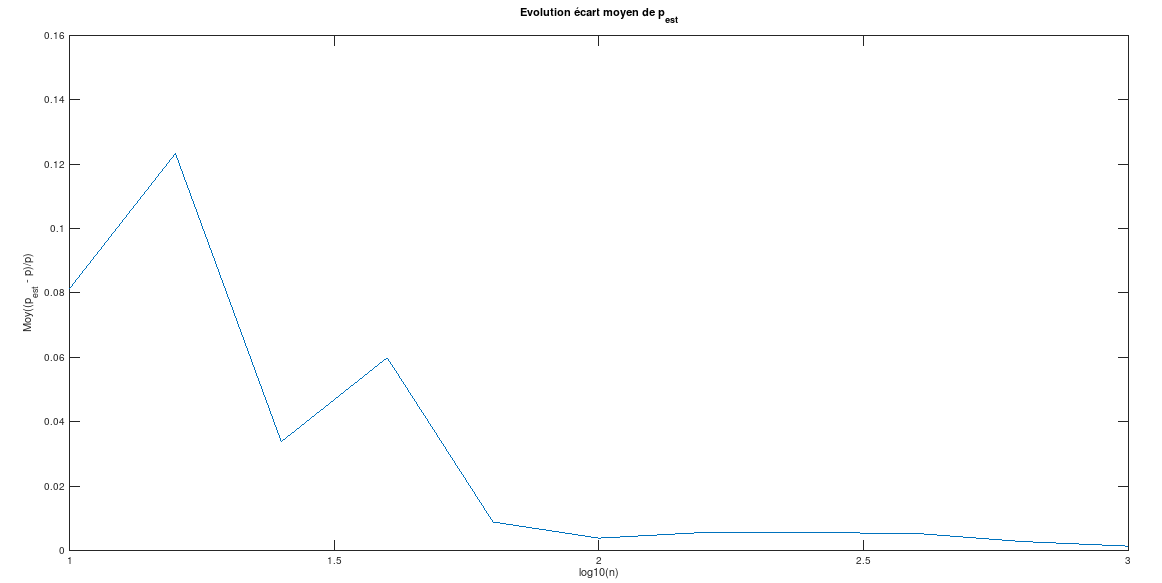
\includegraphics[scale=0.3]{images/biaisMoyGeom.png} 
\end{center}
 \caption{Evolution de l'écart moyen de l'estimateur}
 \label{Evolution de l'écart moyen de de l'estimateur geom}
\end{figure}

On voit très clairement que l'estimateur a un biais positif (en considérant que 500 valeurs permettent de correctement estimer celui-ci, ce qui semble raisonnable) pour des valeurs de n inférieur à 100. On observe 2 pics, le premier à environ +12\% d'erreur pour une taille de 15 et une autre de +6\% pour une taille de 50.

Afin de mieux voir ce biais, on prend un pas de taille de $0.01$ pour $\log_{10}(n)$, n allant de 10 à 100 et on obtient la figure \ref{Evolution de l'ecart moyen de de l'estimateur affiné geom}. Le biais estimé va de +20\% en n=10 et redescend proche 0 en n=100 avec des variations allant jusqu'à 5\% entre chaque estimation. On peut donc raisonnablement affirmer que l'estimateur $\hat{p}$ est biaisé pour des échantillons de taille réduite (en dessous de 100) mais que le biais est suffisamment petit pour des tailles grandes (n>100).

\begin{figure}[!h]
\begin{center}
 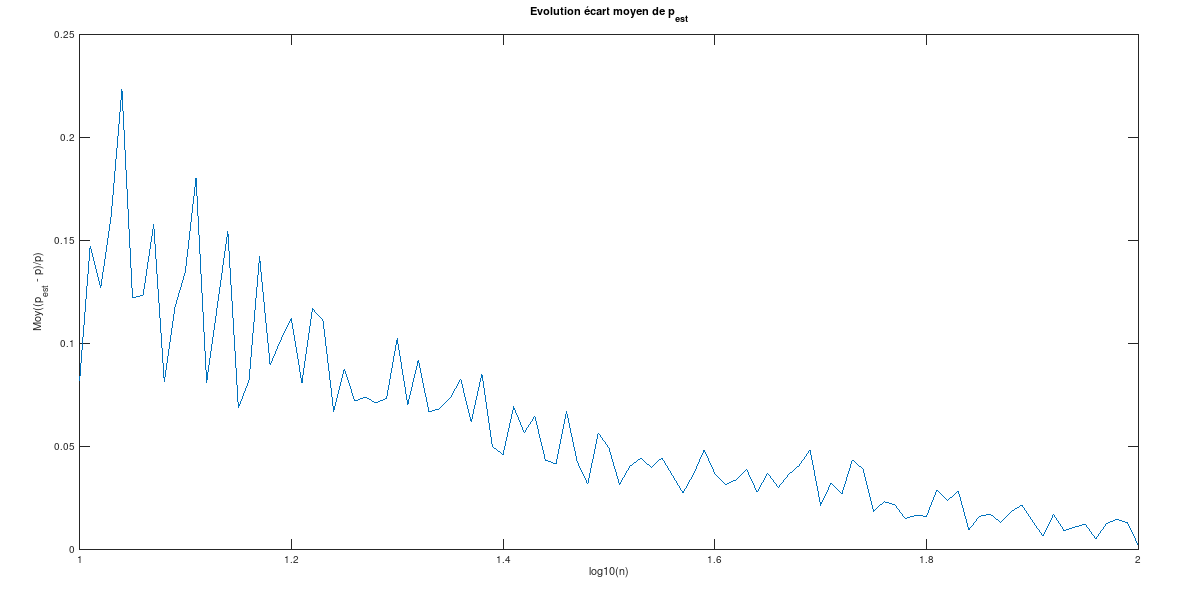
\includegraphics[scale=0.3]{images/biaisMoyGeomBis.png} 
\end{center}
 \caption{Evolution de l'écart moyen de l'estimateur affiné}
 \label{Evolution de l'ecart moyen de de l'estimateur affiné geom}
\end{figure}


\subsection{Loi extrême}

La fonction de répartition extrême de variables indépendantes identiquement distribuées correspond à :
\[F_{X_{\max }}\left( x \right)  = P\left( {{X_{\max }} \le x} \right)\]
\[F_{X_{\max }}  = P\left( {{X_1} \le x,...,{X_n} \le x} \right)\]
\[F_{X_{\max }} = \prod\limits_{i = 1}^n {{F_X}\left( x \right)} \]
\[F_{X_{\max }} = {F_X}\left( x \right)^n\]
Avec une loi géométrique on obtient alors ($k\in{\mathbb{N}_+}$)
\[F_{X_{\max }}(k) = (1-(1-p)^{k})^n\]
Avec la formule du binôme de Newton on a:
\[F_{X_{\max }}(k) = \sum\limits_{l=0}^{n}C^{l}_{n}(p-1)^{kl}\]
Par différence on obtient alors la densité (pour $k>1$, sinon $f_{X_{\max }}(1) = F_{X_{\max }}(1)$) :
\[f_{X_{\max }}(k)=F_{X_{\max }}(k)-F_{X_{\max }}(k-1)\]
\[f_{X_{\max }}(k)=\sum\limits_{l=0}^{n}C^{l}_{n}(p-1)^{kl}-(p-1)^{(k-1)l}\]
\[f_{X_{\max }}(k)=\sum\limits_{l=0}^{n}C^{l}_{n}(p-1)^{kl}(1-(p-1)^{-l})\]


On veut voir à quoi ressemble la loi extrême correspondant à la loi géomètrique. Pour cela on génère $m$ (10, 100, 1000 et 10000) échantillons de $n=100$ variables et on prend la valeur maximale (1\%) de l'échantillon à chaque fois pour générer un échantillon des maximums des échantillons de loi géométrique. On utilise le code Octave suivant :

\lstinputlisting[language=Matlab]{src/extrem.m}

On obtient alors la figure \ref{Distributions extrêmes de la loi géométrique}.

\begin{figure}[!h]
\begin{center}
 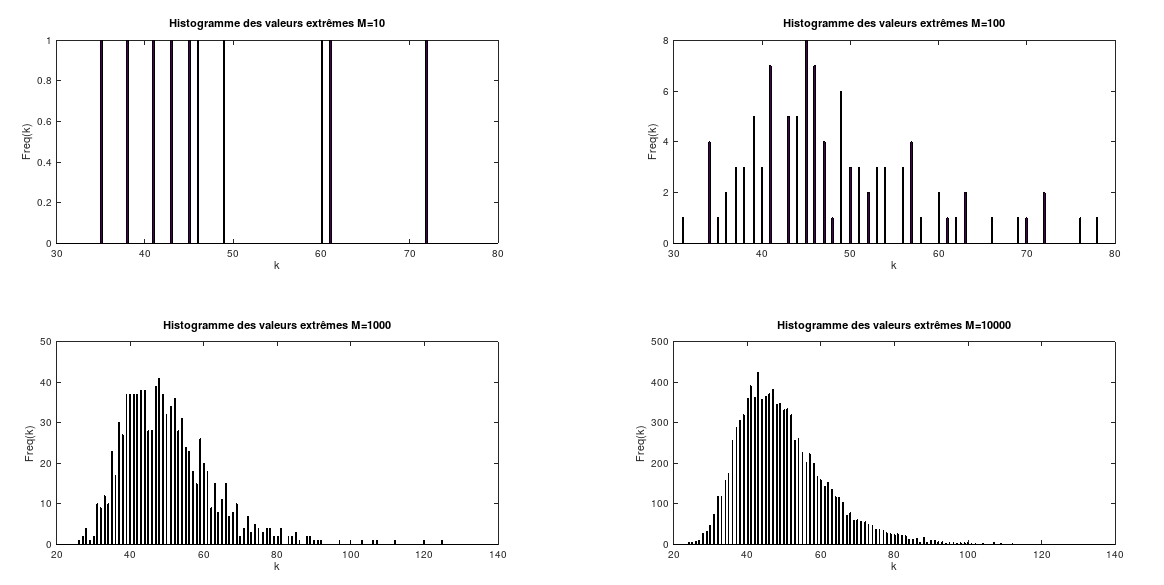
\includegraphics[scale=0.4]{images/extremGeom.png} 
\end{center}
 \caption{Distributions extrêmes de la loi géométrique}
 \label{Distributions extrêmes de la loi géométrique}
\end{figure}

La distribution extrême correspondante ne peut pas être une loi de gumbel puisque nous avons des valeurs uniquement positive. Cela pourrait correspondre à une loi de weibull, de Pareto, lognormale ou encore de Fréchet.
Afin de tester cela on effectue une estimation pour la loi de weibull et la loi lognormale\footnote{les autres lois ne sont pas implémentées et les estimations sont complexes à effectuer} avec le script R suivant (en utilisant la librairie MASS) :

\lstinputlisting[language=R]{src/geomExtrem.R}

On obtient alors la figure \ref{Estimation loi extrême géométrique}. On voit que la loi lognormale donne une très bonne estimation, meilleure que celle de Weibull. Afin de vérifier que la loi lognormale "colle" au données, il faudrait effectuer un test $\chi^2$ pour comparer les données avec la loi théorique ou utiliser un test de normalité comme celui de Shapiro Wilk sur le logarithme des données (mais dans le premier cas il n'y a pas de fonction R directe pour le calcul des intervalles et des probabilités et dans le second cas, R n'accepte pas des échantillons de plus de 5000 (ici on est à 10000)).

\begin{figure}[!h]
\begin{center}
 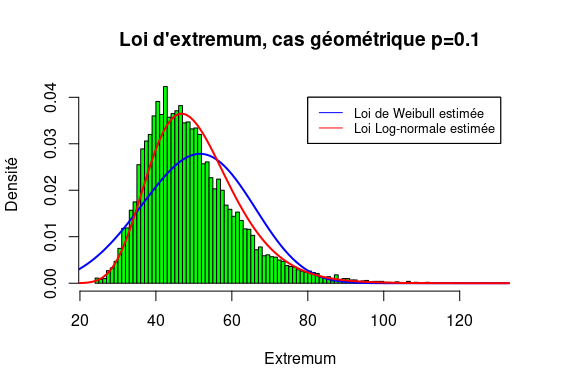
\includegraphics[scale=0.7]{images/RplotGeomExtrem.png} 
\end{center}
 \caption{Estimation loi extrême géométrique}
 \label{Estimation loi extrême géométrique}
\end{figure}



\newpage


\section{Loi de Cauchy}
\subsection{Rappel}
Soit $f_X$ la fonction de densité de Cauchy de deux paramètres $x_0$ et $a$ ($a>0$), définie par:
\begin{equation}
\label{dCauchy}
{f_X}\left( x \right) = \frac{1}{{\pi a\left( {1 + {{\left( {\frac{{x - {x_0}}}{a}} \right)}^2}} \right)}} = \frac{1}{\pi }\frac{a}{{{{\left( {x - {x_0}} \right)}^2} + a}}
\end{equation}

\begin{figure}[h]
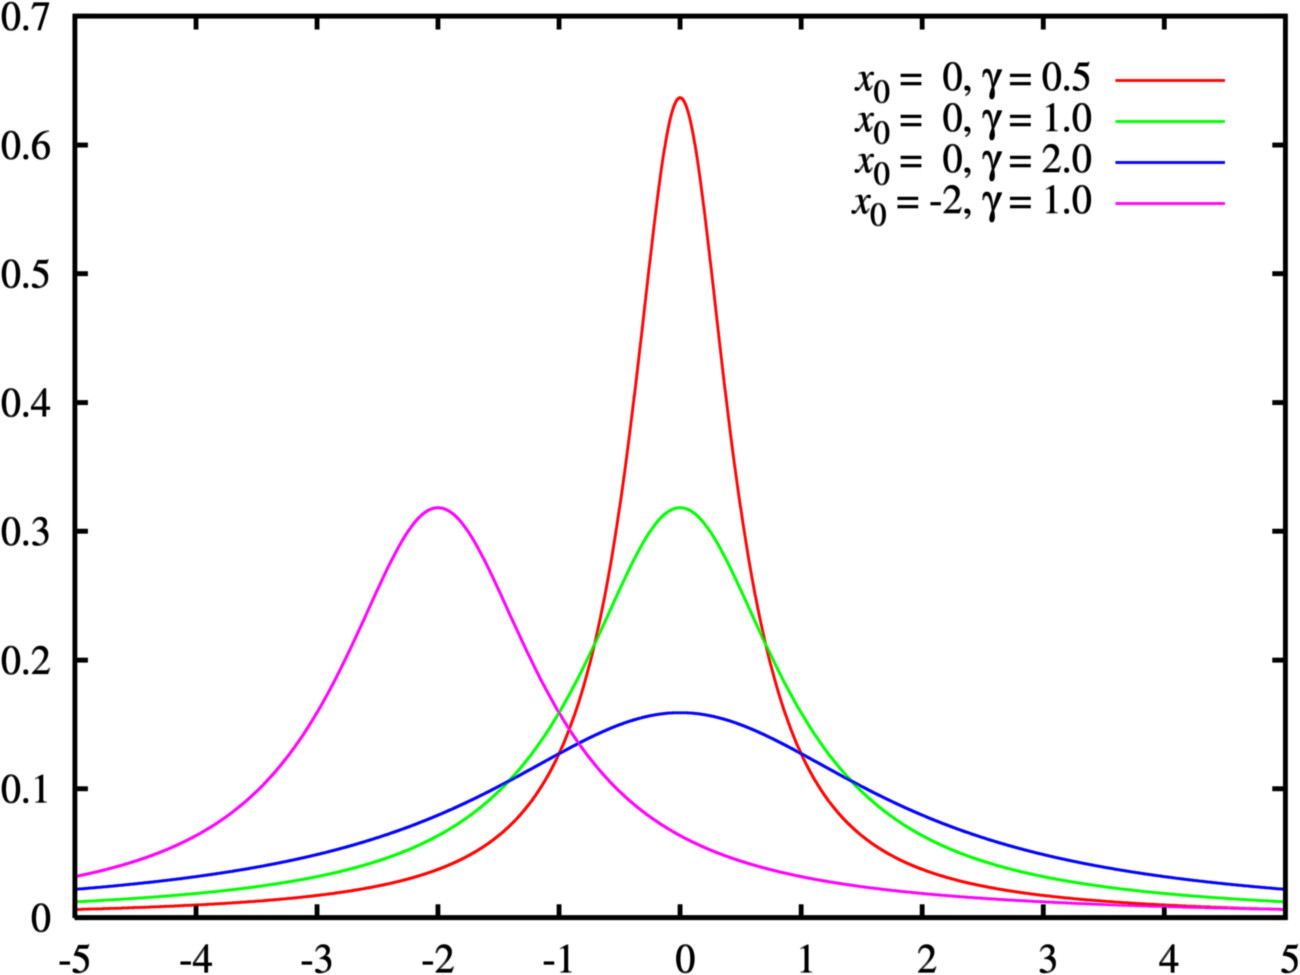
\includegraphics[width=\linewidth]{images/Cauchy_distribution_theoretic.png}
\caption{Distribution théorique de la loi Cauchy. Source : \cite{WikiLoiCauchy}}
\end{figure}

$a$ est dite l'échelle de la fonction, et $x_0$ est sa médiane.

La loi de Cauchy n'admet ni espérance ni écart type.

La fonction de répartition:
\begin{equation}
\label{rCauchy}
{F_X}\left( x \right) = \frac{1}{\pi }\arctan \left( {\frac{{x - {x_0}}}{a}} \right) + \frac{1}{2}
\end{equation}

\subsection{Estimer les paramètres inconnus}

\subsubsection*{Calcul théorique}

Soient $n$ réalisations $x_1, x_2, ..., x_n$. Assumons que ces données suivent la loi de Cauchy \eqref{dCauchy}.

Nous allons utiliser la méthode de maximum de rapport de vraisemblance.

En l'absence d'information de la distribution, nous assumons que ces mesures sont indépendants. Posons une variable aléatoire $X_i$ correspondante à chaque réalisation $x_i$ pour $i=\overline{1, n}$.

On écrit la loi conjointe de ces $n$ variables:

\begin{align*}
L (X) = L\left( {{X_1},{X_2},...,{X_n}} \right) & = \prod\limits_{i = 1}^n {{f_X}\left( {{X_i}} \right)} \\
& = \prod\limits_{i = 1}^n {\frac{1}{\pi }\frac{a}{{{{\left( {{x_i} - {x_0}} \right)}^2} + a}}} \\
& = {\pi ^{ - n}}\prod\limits_{i = 1}^n {\frac{a}{{{{\left( {{x_i} - {x_0}} \right)}^2} + a}}}
\end{align*}

On cherche l'optimum maximale en regardant où s'annule la dérivée de la fonction de vraisemblance
\footnote{On pourrait aussi utiliser le logarithme $\log{L(X)} = \pi^{-n} \sum\limits_{i=1}^{n} \log{a} -
\log{((x_i-x_0)^2+a)}$ qui atteint un optimum au même point puisque cette fonction est continue et strictement croissante
sur $]0;1]$}.

\begin{align*}
\frac{{\partial L}}{{\partial {x_0}}}\left( X \right) & = {\pi ^{ - n}}\sum\limits_{j = 1}^n {\left( { - \frac{{a\left( {2{x_j} - 2{x_0}} \right)}}{{{{\left[ {{{\left( {{x_0} - {x_j}} \right)}^2} + a} \right]}^2}}}\prod\limits_{i = 1;i \ne j}^n {\frac{a}{{{{\left( {{x_i} - {x_0}} \right)}^2} + a}}} } \right)}\\
&  = {\pi ^{ - n}}\left( {\prod\limits_{i = 1}^n {\frac{a}{{{{\left( {{x_i} - {x_0}} \right)}^2} + a}}} } \right)\left( { - \sum\limits_{j = 1}^n {\frac{{2{x_0} - 2{x_j}}}{{{{\left( {{x_0} - {x_j}} \right)}^2} + a}}} } \right) \\
\frac{{\partial L}}{{\partial {x_0}}}\left( X \right) & = 0 \Leftrightarrow \sum\limits_{j = 1}^n {\frac{{{x_0} - {x_j}}}{{{{\left( {{x_0} - {x_j}} \right)}^2} + a}}}  = 0 \text{ : insolvable par la main}
\end{align*}

\begin{align*}
\frac{{\partial L}}{{\partial a}}\left( X \right) & = {\pi ^{ - n}}\sum\limits_{j = 1}^n {\left( {\frac{{{{\left( {{x_j} - {x_0}} \right)}^2} + a - a}}{{{{\left( {{x_j} - {x_0}} \right)}^2} + a}}\prod\limits_{i = 1;i \ne j}^n {\frac{a}{{{{\left( {{x_i} - {x_0}} \right)}^2} + a}}} } \right)}\\
&  = {\pi ^{ - n}}{a^{n - 1}}\frac{{\sum\limits_{j = 1}^n {{{\left( {{x_0} - {x_j}} \right)}^2}} }}{{\prod\limits_{i = 1}^n {\left( {{{\left( {{x_i} - {x_0}} \right)}^2} + a} \right)} }} > 0,\ \forall a > 0
\end{align*}
On ne peut donc pas estimer a par la méthode du maximum de vraisemblance.

\subsubsection*{Résolution par R}

On génère un échantillon avec $a$ et $x_0$ au choix. Puis, on utilise la fonction $mle$ (Maximum Likelihood Estimator) de librairie \emph{stats4} avec 2 valeurs initiales $\hat{a}$ et $\hat{x_0}$ pour estimer $a$ et $x_0$.

Nous essayons d'estimer $x_0$ et $a$ directment. L'algorithme d'approximation implémenté dans R a besoin d'un bon point de départ, sinon le résultat obtenu variera grossièrement.
\begin{itemize}
\item Etant donné que la médiane est théoriquement aussi $x_0$, choisissons $x_0$ comme la médiane de l'échantillon.
\item Nous avons ${f_X}\left( {{x_0}} \right) = \frac{1}{{\pi a}}$. En plus, $f_X(x_0)$ est la valeur maximale $d$ de densité. Prenons alors $\hat a = \frac{1}{{\pi d}}$.
\end{itemize}

Testons avec $x_0=13$ et $a=0.5$.

%PROBLEME UTF8 Cauchy.R
\lstinputlisting[firstline=2, lastline=50, language=R]{src/Cauchy.R}

\begin{figure}[h]
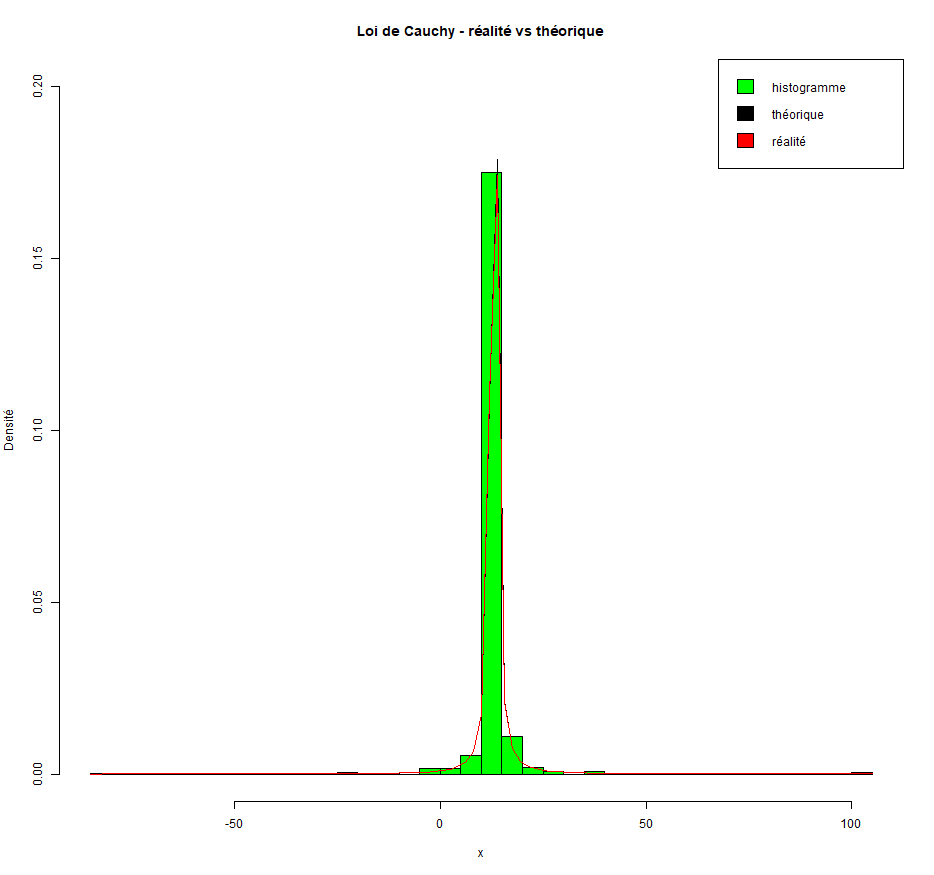
\includegraphics[width=\linewidth]{images/Cauchy_real_vs_theo.png}
\caption{Représentation de l'histogramme et de la courbe de densité}
\end{figure}

Pour $x_0=13$ et $a=0.5$, les valeurs trouvées par R sont $\hat{x_0} = 12.9877139$ et $\hat{a} = 0.4951073$.

\subsection{Test de paramètres}

Nous testons ici si les valeurs trouvées par R sont vraiment approchées à celles théoriques. Pour l'instant, nous n'avons pas d'outils pour vérifier 2 variables en couple.

\subsection{Test d'adéquation}

R nous donne la fonction \emph{ks.test} pour valider la compatibilité d'une échantillon avec une loi selon le test de Kolmogorov-Smirnov.

\lstinputlisting[firstline=52, lastline=52]{src/Cauchy.R}

On a trouvé $D = 0.02696$, $p-value = 0.4614$, ce la signifie que l'écart maximale est $0.02696$ et le niveau d'acceptation est $0.4614$. Vu que nous fixons $\alpha = 5\% < p-value$, l'échantillon dépasse largement le test. Autrement dit, il se distribue selon la loi de Cauchy.

\subsection{Etude de biais d'estimateur}

Maintenant on s'intéresse au biais d'estimateur. On relance l'algorithme en-dessus avec de différents observations ($N = 100, 125, 150,..., 1100$). $x_0 = 13$ et $a = 0.5$.

\lstinputlisting{src/Cauchy-variN.R}

\begin{figure}[!h]
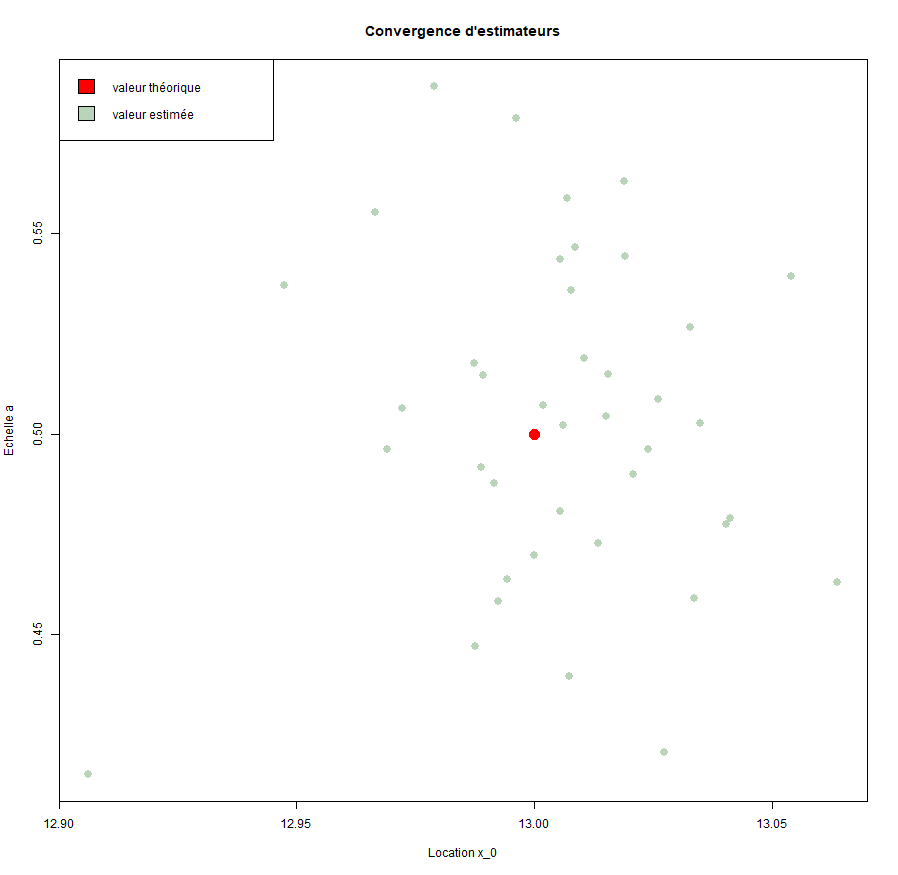
\includegraphics[width=\linewidth]{images/Cauchy_convergence_parametres.png}
\caption{Convergences de $\hat{x_0}$ et $\hat{a}$ vers valeurs théoriques}
\end{figure}

Nous observons que les valeurs estimées se rassemblent  proche de la valeur théorique.
\clearpage
\subsection{Etude de loi d'extremum}

Générons donc des échantillons de $n$ valeurs ($n=10, 100, 1000, etc.$). Parmi chacun, $\frac{n}{10}$ valeurs les plus grandes seront gardées pour étudier la loi d'extremum.

Comme les réalisations sont indépendantes et identiquement distribuées, théoriquement:
\begin{align*}
{F_{{x_{\max }}}}\left( x \right) & = P\left( {{X_{\max }} \le x} \right)\\
&  = P\left( {{X_1} \le x,...,{X_n} \le x} \right)\\
 & = \prod\limits_{i = 1}^n {{F_X}\left( x \right)} \\
 & = {F_X}{\left( x \right)^n}
\end{align*}

Avec ${F_X}\left( x \right) = \frac{1}{\pi }\arctan \frac{{x - {x_0}}}{a} + \frac{1}{2}$, la fonction de répartition de la loi de Cauchy. Alors, \[{F_{{x_{\max }}}}\left( x \right) = {\left( {\frac{1}{\pi }\arctan \frac{{x - {x_0}}}{a} + \frac{1}{2}} \right)^n}\]

Or, \[\left| {\arctan \frac{{x - {x_0}}}{a}} \right| < \frac{\pi }{2} \Rightarrow \frac{{ - \pi }}{2} < \arctan \frac{{x - {x_0}}}{a} < \frac{\pi }{2} \Rightarrow 0 < \arctan \frac{{x - {x_0}}}{a} + \frac{\pi }{2} < \pi \]

Par conséquent,

\[\begin{array}{l}
\tan \left( {\arctan \frac{{x - {x_0}}}{a} + \frac{\pi }{2}} \right) =  - \cot \left( {\arctan \frac{{x - {x_0}}}{a}} \right) =  - \frac{a}{{x - {x_0}}}\\
 \Rightarrow \arctan \frac{{x - {x_0}}}{a} + \frac{\pi }{2} = \arctan \left( { - \frac{a}{{x - {x_0}}}} \right) = \arctan \frac{a}{{{x_0} - x}}\\
 \Rightarrow {F_{{x_{\max }}}}\left( x \right) = {\pi ^{ - n}}{\left( {\arctan \frac{{x - {x_0}}}{a} + \frac{\pi }{2}} \right)^n} = {\pi ^{ - n}}{\arctan ^n}\frac{a}{{{x_0} - x}}
\end{array}\]

Nous prenons 3 valeurs les plus grandes pour chaque itération, et établissons leur histogramme.

%PROBLEME UTF8 Cauchy-extreme.R
\lstinputlisting[language=R, firstline=2, lastline=40]{src/Cauchy-extreme.R}


\begin{figure}[!h]
\centering
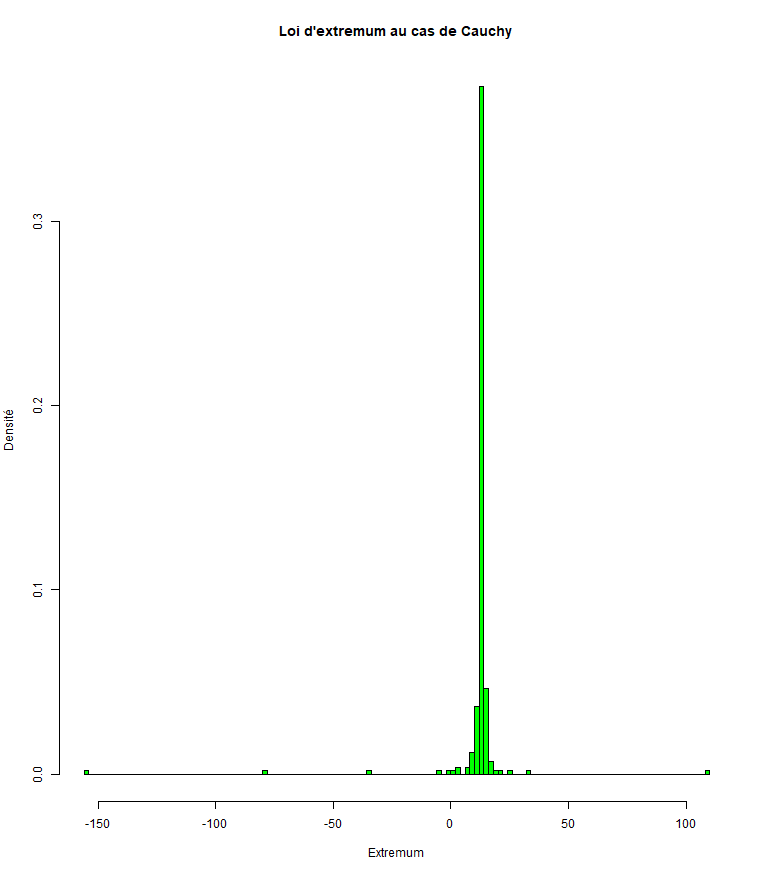
\includegraphics[width=0.8\linewidth]{images/Cauchy_extremum.png}
\caption{Histogramme de valeurs extremum de la distribution de Cauchy}
\end{figure}


\clearpage

\begin{thebibliography}{3}
\bibitem{WikiLoiCauchy}

Wikipedia,

\url{https://en.wikipedia.org/wiki/Cauchy_distribution}

\bibitem{LoiExtremum} 
\url{https://en.wikipedia.org/wiki/Generalized_extreme_value_distribution}

\end{thebibliography}
\end{document}
